\documentclass[11pt,a4paper,fleqn]{article} 
%%%%% general %%%%%
\usepackage[T1]{fontenc} 
\usepackage{geometry}
\geometry{a4paper, top=20mm, left=20mm, right=20mm, bottom=20mm,headsep=10mm, footskip=12mm}
\usepackage[singlespacing]{setspace} %Zeilenabstand
\usepackage{xspace} %Befehle fuer Bezeichner, damit danach Leerzeichen
%%%%% lists %%%%%%

\usepackage[alwaysadjust,flushleft]{paralist}
\usepackage{enumerate}
%%%%% graphics and tables %%%%%
%\usepackage{graphicx}
\usepackage{subfigure}
\usepackage{booktabs}
\usepackage{multirow}

%\usepackage{longtable}
\usepackage{rotating}
%\usepackage{placeins}
\usepackage{flafter} %no floating object appears in the text above the position where it is defined
%\usepackage[font=small,labelfont=bf]{caption} 
\newcommand{\ra}[1]{\renewcommand{\arraystretch}{#1}}
\usepackage{tikz}
\usepackage{pgfplots}

%%%%% Mark changes %%%%%
%\usepackage{soul}
%\setstcolor{red}
%\usepackage{cancel}
\usepackage[final]{changes}

%%%%% bibliography %%%%%
\usepackage{natbib}
\bibliographystyle{abbrvnat}
\bibpunct[, ]{(}{)}{,}{a}{}{,}%
\def\bibfont{\small}%
\def\bibsep{\smallskipamount}%
\def\bibhang{24pt}%
\def\newblock{\ }%
\def\BIBand{and}%
%%%%% math and algorithms %%%%%
\usepackage{amsmath}
\usepackage{amssymb}
%\usepackage{algorithm}
\usepackage{array}
%\newcolumntype{H}{>{\setbox0=\hbox\bgroup}c<{\egroup}@{}}
\usepackage{algorithmic}
\usepackage{fixltx2e} % text super and subscripts
%%%%% color %%%%%%
\PassOptionsToPackage{usenames,dvipsnames}{color}
%\usepackage[usenames,dvipsnames]{color}
%%%%% hyperref %%%%%%
%\usepackage{url}
%\usepackage{preview}
%\usepackage{breakurl} \% break long urls
%\usepackage[colorlinks,linkcolor=Goldenrod,citecolor=Brown]{hyperref}
\usepackage{hyperref}
% \hypersetup{
%     bookmarks=true,
%     unicode=false,
%     pdftoolbar=true,
%     pdfmenubar=true,
%     pdffitwindow=false,
%     pdfstartview={FitH},
%     pdftitle={My title},
%     pdfauthor={Author},
%     pdfsubject={Subject},
%     pdfcreator={Creator},
%     pdfproducer={Producer},
%     pdfkeywords={keyword1} {key2} {key3},
%     pdfnewwindow=true,
%     colorlinks=true,
%     linkcolor=black,
%     citecolor=black,
%     filecolor=black,
%     urlcolor=black
% }


\pgfplotsset{compat=1.12}
\allowdisplaybreaks[4]
%%%%% Math Operators %%%%%
\DeclareMathOperator*{\argmin}{arg\,min}
\DeclareMathOperator*{\argmax}{arg\,max}

\usepackage{atbegshi}% http://ctan.org/pkg/atbegshi
\AtBeginDocument{\AtBeginShipoutNext{\AtBeginShipoutDiscard}}


\begin{document}

\onehalfspacing
\title{Optimizing Air Cargo Handling at an International Airline Hub for AbOvo \\} 
\author{Ilkim Canoler \\ Luckshan Sivakumar \\  Nikhil Kulkarni \\ Karthikeyan Ramasubbu \\ Shekhar Dure}
$\newline$
$\newline$
\date{12th June 2019}
\maketitle
\thispagestyle{empty}


$\newline$
\begin{abstract}
	In this study, we solve an operational planning problem in the air cargo industry. In an international airline hub, all shipments which are arrived at airport, go through several processes such as breaking down and building up. At the end, all have to catch their connection flight on time. Due to the complexity of the overall puzzle, current practices at airlines are to split up the puzzle into two smaller and thus simpler puzzles. The goal of this case is to solve the full planning problem simultaneously or when solving separately considering the dependencies between the two parts. Working with our industrial partner AbOvo, we provide a comprehensive overview of the air cargo planning problem. We formalize its requirements and the objectives. Furthermore, we develop and evaluate suitable solution approaches. We solve the full planning problem simultaneously by using integer linear programming and make all individual shipments catch their related connection flights on time.
	
\end{abstract}

\clearpage
\pagenumbering{arabic} 

\newpage

\tableofcontents

\newpage

\section{Introduction}
\label{sec:introduction}

$\newline$
An international airline hub needs to plan the air cargo movement so that all shipments catch their connecting flights or road connections. Air cargo shipments are transported in so-called unit load devices (ULDs). It allows a large quantity of cargo to be bundled into a single unit like a pallet or a container. A ULD may contain many shipments which need to go different final destinations. Hence, at the first step of the whole process in Figure 1, the incoming ULDs are broken down on arrival. Here in the breakdown zone (BD), ULDs have to be unpacked and seperated. The seperate shipments are transported to the warehouse to wait for the build up call. These shipments are then moved to the packing area which is called buildup zone (BU). At the end, outbound ULDs are constructed from these shipments, and they are taken to the outbound flight for loading. All zones have different attributes such as the number of workstations, capacities, transportation times between zones and the warehouse. Shipments also have different attributes such as priority and weight. Regarding all the attributes, constraints and the parameters which are stated in detail in the problem description section, the goal of the optimization process is to build up all ULDs as soon as possible to make them catch their connections.

%\noindent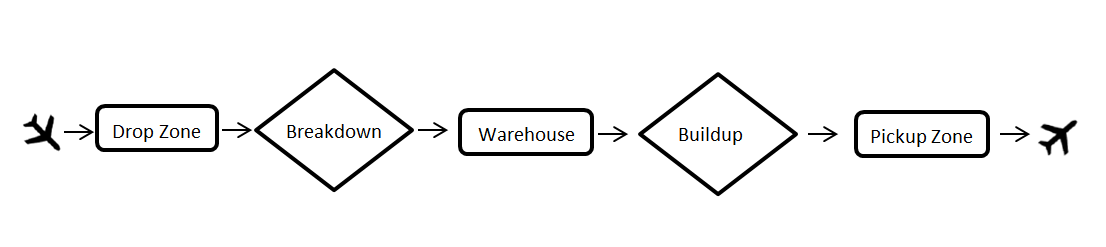
\includegraphics[width=18cm]{1_process.png}\qquad

\begin{figure}[hbt!]
	\centering
	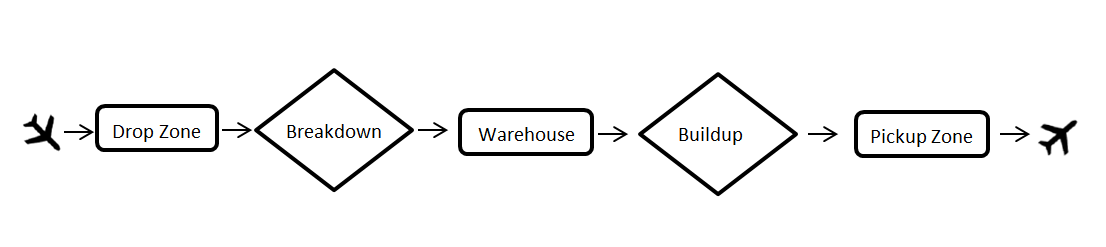
\includegraphics[width=170mm,scale=1.5]{1_process.png}
	\caption{The Process That Takes Place at a Hub}
	\label{fig:The Process That Takes Place at a Hub}
\end{figure}

\section{Problem Description}
\label{sec:problemdescription}

$\newline$
The whole handling process of one shipment begins in the drop zones when it comes to the airport in an inbound ULD. There are 4 drop zones in the airport. ULDs are unloaded from an aircraft by the ground handling agent and placed in one of the drop zones (not part of our planning problem). Each drop zone has different number of workstations. Each ULD has a scheduled arrival and at a later stage an actual arrival time. From the drop zone, each ULD has to be taken to the breakdown zone to get unpacked. Our problem starts here. There are different distances between each drop zone and each breakdown zone. 

%The sample distances between some of the drop zones and some of the BD zones are given below in the Figure 2.

%\newpage

%\noindent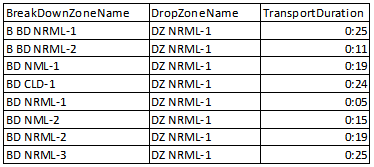
\includegraphics[width=12cm]{distances_drop_bdzone.png}\qquad

%\begin{figure}[hbt!]
%	\centering
%	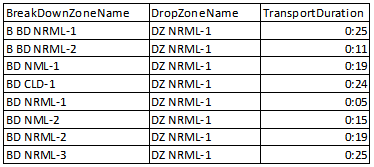
\includegraphics[width=100mm,scale=1.5]{distances_drop_bdzone.png}
%	\caption{Sample Distances Between Drop Zone and Break Down Zone}
%	\label{fig:Sample Distances Between Drop Zone and Break Down Zone}
%\end{figure}

$\newline$
In BD zone, ULDs are seperated into shipments. There are 12 different BD zones in the hub that are located at different places of the airport. Thus all BD zones have different attributes. Attributes related to BD zones are: 

\begin{itemize}
	\item Different characteristics for each BD zone for example some of the BD zones are for animals, some of them are for cooled products and the others are normal BD zones.
	\item Different number of workstations within the BD zone.
	\item Different transportation times to the warehouse.
	\item Different handling times per ULD.
\end{itemize}

%\begin{figure}[hbt!]
%	\centering
%	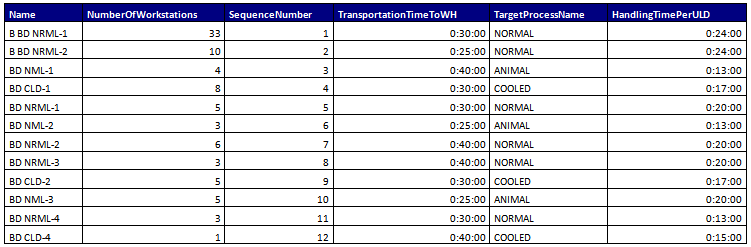
\includegraphics[width=150mm,scale=1.0]{BDZones.png}
%	\caption{Break Down Zone Attributes}
%	\label{fig:Break Down Zone Attributes}
%\end{figure}

%\noindent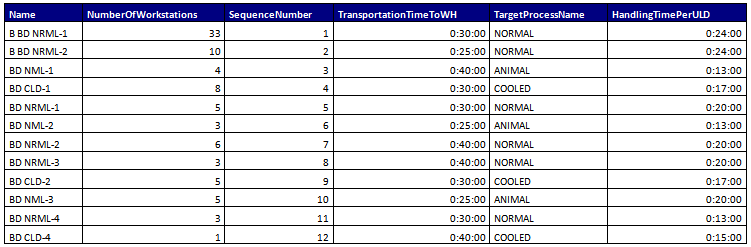
\includegraphics[width=30cm]{BDZones.png}\qquad

Within the BD zone, the decision needs to be taken in which order the ULDs should be unpacked. ULDs need to be broken down early enough, so all shipments can make their connections or promised pickup time. There are 3 different shipments within the hub. Cooled products, normal products and animals. Each shipment has different priority in the BD zones. For example, animals or cooled products need to be processed before the regular shipments. ULDs that contain a shipment with a high priority need to be unpacked earlier than the others. Each shipment in transit within the ULD needs to catch the connecting flight. When the shipments are unpacked, depending on the scheduled departure time of the connection flight on which cargo is booked, it is either stored temporarily in the warehouse or directly sent to the build up process. The warehouse (WH) is fully automated and with the assumption, that there are never capacity constraints in the WH. As soon as enough stock is available in the storage WH to build up one ULD for a specific aircraft, these can be requested to be provided to the BU zone.

$\newline$
In a next step the shipments are built up again to ULDs depending on their connecting flight. This is done within a build up zone (BU zone). A departing aircraft type has a link to a specific BU zone, so with the provided information which aircraft the shipment should go on, the BU zone is known. Here again a shipment with a high priority has to be built up earlier then the other shipments. There are 8 different BU zones and each BU zone has different number of workstations within. At each work station one ULD can be built up at the same time. The shipments are provided from the storage WH to the chosen work station. If the building up of two ULDs for the same aircraft are planned at one work station, it is not allowed to build up a ULD for a different aircraft in between, even if there is some idle time. The reason is that after building up one ULD there might be some shipments with the same destination left. It should be avoided to move those around, so they would stay at the work station for the build up of the next ULD for the same aircraft. From each BU zone, there are different transportation times to each flight. In addition to this, there are different default processing times for each flight which is also given in the data. This means each ULD has additional processing time before the regarding flight. Here for all ULDs, the capacity is the same which is 400 kg. For some of the flights, there is a pre-processing buffer time necessary to consider. Sample tables related to these characteristics are given below for a clear understanding:

\begin{itemize}
	\item Different handling times and transport times from the WH for each BU zone.
	
	%\begin{figure}[hbt!]
	%	\centering
	%	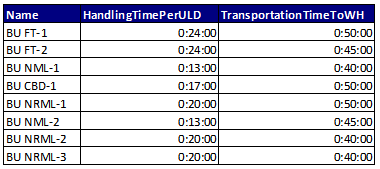
\includegraphics[width=100mm,scale=1.5]{buzone_data1.png}
	%	\caption{Handling Times and Transportation Times from Warehouse to BU Zones}
	%	\label{fig:Handling Times and Transportation Times from Warehouse to BU Zones}
	%\end{figure}

\end{itemize}

	%%\noindent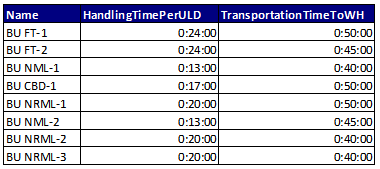
\includegraphics[width=14cm]{buzone_data1.png}\qquad

\begin{itemize}

	\item Sample workstations within some BU zones.
	
%	\begin{figure}[hbt!]
	%	\centering
	%	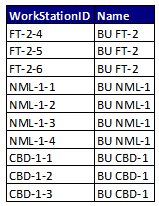
\includegraphics[width=40mm,scale=1.0]{sample_ws_bu.png}
	%	\caption{Workstations in BU Zones}
	%	\label{fig:Workstations in BU Zones}
%	\end{figure}
	%%\noindent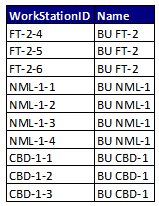
\includegraphics[width=8cm]{sample_ws_bu.png}\qquad

\end{itemize}

\begin{itemize}

	\item Sample flights related to some BU zones and the transportation time between the flight and the BU zone.
	
	%\begin{figure}[hbt!]
	%	\centering
	%	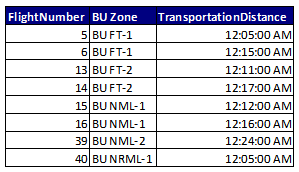
\includegraphics[width=90mm,scale=1.5]{sample_bu_flight.png}
	%	\caption{Sample Flights Related to BU Zones and Transpotation Times}
	%	\label{fig:Sample Flights Related to BU Zones and Transpotation Times}
%	\end{figure}
	%%\noindent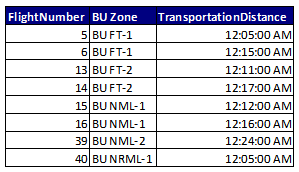
\includegraphics[width=10cm]{sample_bu_flight.png}\qquad

\end{itemize}

\begin{itemize}

	\item Pre-processing buffer times for the flights.
	
	%\begin{figure}[hbt!]
	%	\centering
	%	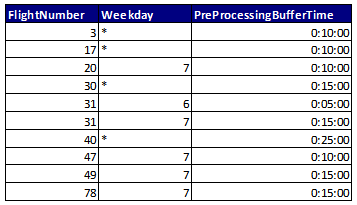
\includegraphics[width=90mm,scale=1.5]{preprocess_time.png}
	%	\caption{Pre-Processing Times of the Flights}
	%	\label{fig:Pre-Processing Times of the Flights}
%	\end{figure}
	%%\noindent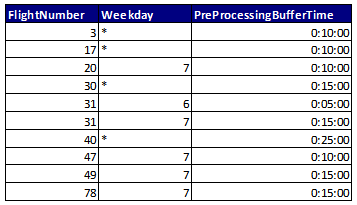
\includegraphics[width=10cm]{preprocess_time.png}\qquad
	
\end{itemize}

The goal is to build up all ULDs as soon as possible to make the connections, while the work should be processed in batches, to avoid unnecessary transportation within the BU zone.

%\newpage


\section{Mathematical Model for the Problem}
\label{sec:mathmodel}

Our mathematical model for this problem is a combination of two puzzles, which are Break Down Zone and the Build Up Zone assignments. The overall view of the general process can be seen in Figure 2 below.

$\newline$ 

\begin{figure}[hbt!]
	\centering
	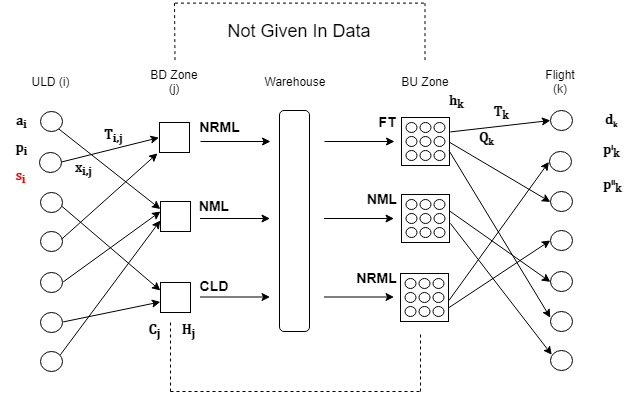
\includegraphics[width=170mm,scale=1.5]{Aircargo_overall.png}
	\caption{Overall View for The Aircargo Process}
	\label{fig:Overall View for The Aircargo Process}
\end{figure}

\subsection{Break Down Process}
\label{sec:ParamBDZone}

In BD zones, our model has arrival time parameters for each ULD. Similar to this, each BD zone has its own capacity, handling time and transportation time from drop zone. Each ULD is a part of the ULD set I and each BD zone is a part of the BD zones set J. Time is discretized into minutes in set T.

\begin{equation*} ${\color{black} ULD i}$ {}  \in {}  ${\color{black}I}$ {} = {} ${\color{black}\{1,2,3,...,N\}}$  \end{equation*} 
\begin{equation*} ${\color{black} BD zone j}$ {}  \in {}  ${\color{black}J}$ {} = {} ${\color{black}\{1,2,3,...,M\}}$ \end{equation*} 
\begin{equation*} ${\color{black} Time horizon t}$ {}  \in {}  ${\color{black}T}$ {} = {} ${\color{black}\{1,2,3,...,T\}}$ \end{equation*}
\begin{equation*} ${\color{black} Shipments l in ULD i}$ {}  \in {}  ${\color{black}Li}$ {} = {} ${\color{black}\{1,2,3....,L\}}$ \end{equation*} %newly_added_by_ilkim% 


${\color{black}a_{i}}$ : Arrival time of ULD ${\color{black}i}$ in drop zone 

${\color{black}d_{i}}$ : Earliest Departure time of a shipment in ULD ${\color{black}i}$ 

%$\textcolor{black}{s_{i}}$ : Idle time spent by ULD ${\color{black}i}$ in drop zone

%$\textcolor{black}{p_{i}}$ : Priority of ULD ${\color{black}i}$

${\color{black}c_{j}}$ : Capacity of BD zone ${\color{black}j}$

$\textcolor{black}{h_{j}}$ : Handling time in BD zone ${\color{black}j}$

$\textcolor{black}{T_{ij}}$ : Time taken to transport an ULD ${\color{black}i}$ to BD zone ${\color{black}j}$

$\textcolor{black}{T_{j}}$ : Time taken to transport shipments from ${\color{black}i}$ to BD zone ${\color{black}j}$ to Warehouse


\subsubsection{Decision Variables for Break Down Process}
\label{sec:DVBDZone}

In the Break Down zone, the decision needs to be taken which ULDs should be assigned to which BD zone at which time. For this reason, the decision variable has to be binary. 1 for the ULD i is assigned to BD zone j at time t, 0 for the ULD i is not assigned to BD zone j at time t. 

$\newline$

$\textcolor{black}{x_{ij}^{t}\in\{0,1\}, \forall {i \in I, j \in J, t \in T}}$ : if a ULD i is assigned to BD zone j at time t or not.


\subsubsection{Constraints for Break Down Process}
\label{sec:constraintsBDZone}

For BD zone processes we have several constraints. The first one (1) is the constraint that ensures that the ULD is assigned at a feasible time, the second one (2) is an assignment constraint which means all ULDs have to be assigned to exactly one BD zone.

$\newline$
The time at which Break down of  ULD i starts, $t_{i,start} = \sum_{j \in J}\sum_{t=a_{i}}^{d_{i}} t . x_{ij}^t $
$\newline$
$\newline$
Each ULD takes i  $T_{ij}$ time to travel to its assigned BD zone j, therefore the following constraint ensures that the start time of ULD i is greater than the sum of its arrival time and transportation time :
$\newline$
\begin{align}
\sum_{j \in J}\sum_{t=a_{i}}^{d_{i}} (t- T_{ij}) . x_{ij}^t \ge a_{i} ,  \qquad \forall i \in I
\end{align}

Each ULD i must be assigned to a BD zone j before the earliest departure time of the shipment it contains. We will further tighten this time limit in other constraints that follow. The following constraint ensures that each ULD is assigned : 

\begin{align}
\sum_{j \in J}\sum_{t=a_{i}}^{d_{i}} x_{ij}^{t} = 1 \qquad \forall i \in I
\end{align}

For the special case given in this problem, where we have multiple drop zones, the each ULD has to be assigned to multiple BD zones associated with it. In the constraints (3) and (4), we assign such multiple drop zone ULDs to their respective BD zones i.e animal BD zone and normal BD zone.
\begin{align}
\sum_{j \in J_{NML}}\sum_{t=a_{i}}^{d_{i}} x_{ij}^{t} = 1 \qquad \forall i \in I
\end{align}

\begin{align}
\sum_{j \in J_{NRML}}\sum_{t=a_{i}}^{d_{i}} x_{ij}^{t} = 1 \qquad \forall i \in I
\end{align}

In the fifth consraint (5), we say that for multiple drop zone ULDs, animal BD zone has to be assigned before the regular shipment BD zone.

$J_{NML} \bigcup J_{NRML} = J$

\begin{align}
\sum_{j\in J_{NML}}\sum_{t=a_{i}}^{d_{i}} (t + h_{j}) . x_{ij}^t  \le \sum_{j\in J_{NRML}}\sum_{t=a_{i}}^{d_{i}} (t) . x_{ij}^t
\end{align}


$\newline$
The sixth one (6) is the capacity constraint. In the sixth constraint (6), we say that if ULD's in subset i are started to be processed at time t, no more ULDs than the remaining capacity of the BD zone j can start before $t + h_{j}$ , because the process of breaking down the current ULDs needs to be completed.
If ULDs in subset i start at t in BD zone j, then other ULDs are in $u \in I \setminus \{i\}$. In the first part of the constraint, we are calculating the remaining capacity for the BD zone at time t . For the second part of the constraint, we are stating that whatever will be assigned in next time period $t + h_{j}$ should be less than or equal to remaining capacity.

\begin{align}
c_{j} - \sum_{i \in I} x_{ij}^{t} \ge \sum_{u \in I \setminus \{i\}}\sum_{\tau = t+1}^{t+h_{j}-1} x_{ij}^{\tau} \qquad \forall t \in T, \forall j \in J
\end{align}

$\newline$
The effect is no more ULDs than the capacity of BD zone are assigned at any time.
$\newline$
$\newline$

ULD i is broken down at time, $t_{i,end} =   \sum_{j \in J}\sum_{t=a_{i}}^{d_{i}}{\color{black}{(t + h_{j})}} . x_{ij}^t$

$\newline$
Lets consider the journey of each shipment as in Figure 3 shown below. Each ULD i has $l \in L_{i}$ shipments in it. If ULD i is assigned at time t to BD zone j, then $x_{ij}^t = 1$ and it also means that all shipments in ULD i are assigned at that time t to BD zone j.


\begin{figure}[hbt!]
	\centering
	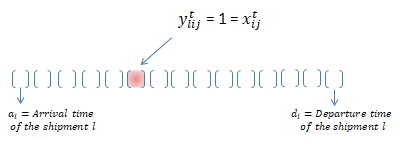
\includegraphics[width=130mm,scale=1.5]{Marco.png}
	\caption{Journey of Shipment}
	\label{fig:Journey of Shipment}
\end{figure}

\subsection{Build Up Process}
\label{sec:ParamBUZone}

We define parameters for flights and Build up zones :

\begin{equation*} ${\color{black} Flight k}$ {}  \in {}  ${\color{black}K}$ {} = {} ${\color{black}\{1,2,3,...,K\}}$  \end{equation*} 
\begin{equation*} ${\color{black} BU zone for flight k has Workstations m}$ {}  \in {}  M_k {} = {} ${\color{black}\{1,2..,M\}}$  \end{equation*}
\begin{equation*} ${\color{black} Capacity of ULD in Kgs (W)}$  = 400 \end{equation*}
\begin{equation*} ${\color{black} Weight of each shipment}$  = w_l \end{equation*}
\begin{equation*} ${\color{black} Time taken to build up a ULD in BU zone for Flight k}$  = b_k \end{equation*}
\begin{equation*} ${\color{black} Pre-processing time for each Flight k}$  = p_k \end{equation*}

\subsubsection{Decision Variables for Build Up Process}
\label{sec:DVBDZone}

In the Build Up zone model, the decision needs to be taken regarding which shipments should be assigned to which workstation at what time in a given Build Up zone. For this reason, we introduce a decision variable:  ${z_{lm}^{t}}$

$\newline$
Shipment  \textcolor{black}{$l$} having departure flight  \textcolor{black}{$k$} is assigned to one of  \textcolor{black}{$"m"$} workstations in its BU Zone.
$\newline$

$\textcolor{black}{z_{lm}^{t}\in\{0,1\}, \forall {i \in I, l \in L_i, m \in M_k, t \in T}}$
$\newline$


$\newline$
${Q_{mk}^{t}}$ is our binary decision variable to decide if the the Workstation m is assigned to build ULD for Flight k at time t or not. 
$\newline$

$\textcolor{black}{Q_{mk}^{t}\in\{0,1\}, \forall {k \in K, m \in M_k, t \in T}}$
$\newline$
\subsubsection{Constraints for Build Up Process}
\label{sec:constraintsBUZone}

All shipments must be assigned to a workstation in its designated Build up zone.
$\newline$
\begin{align}
\sum_{m \in M}\sum_{t=a_{l}}^{d_l} z_{lm}^{t} = 1  \qquad \forall k \in K, \forall l \in L_k  
\end{align}

$\newline$
If shipments in subset  $\textcolor{black}{l\in\ L_k }$ start at $\textcolor{black}{t}$ in $\textcolor{black}{m^{th}}$  workstation, other shipments in subset $\textcolor{black}{p\in\ L_k \setminus \{ l\} }$ cannot start before $\textcolor{black}{t}$ + $\textcolor{black}{b_{k}}$
$\newline$

\begin{align}
Q_{mk}^{t}.W - \sum_{l\in L_k}z_{lm}^{t}.w_l \ge  \sum_{p\in L_k\setminus \{ l\}}            \sum_{\tau=t+1}^{t+b_k-1} z_{pm}^{\tau}.w_l , \qquad \forall k \in K, \forall m \in M_k, \forall t \in T  
\end{align}


$\newline$

The number of workstation in the Build up zone that are to be assigned to build ULDs for flight k shall not exceed the number of ULDs that go into the flight and hence we need the following constraint to take care of this.
$\newline$

\begin{align}
\sum_{m \in M_k}\sum_{t=a_l}^{d_k}{Q_{mk}^{t}} \le \dfrac{\sum_{l \in L_k}\sum_{m \in M}\sum_{t=a_l}^{d_k}{z_{lm}^{t} w_{l}}}{W} + 1 ,  \qquad \forall k \in K
\end{align}

$\newline$
If a workstation 'm' in a buildup zone is assigned to flight k at time t, then no other flight can start building its ULDs in that workstation before time t+bk.

$\newline$
\begin{align}
1 - {Q_{mk}^{t}} \ge \sum_{q \in K \setminus \{k\}}  \sum_{\tau = t}^{t + b_{k}}{Q_{mq}^{t}} ,  \qquad \forall k \in K , \forall m \in M_{k}, \forall t \in T
\end{align}

%\subsubsection{Precedence constraints}
%\label{sec:ParamBUZone}

In the entire timeline of a shipment from its arrival to departure as in Figure 4, we have a precedence contraint on processes a shipment goes through. The Break down process preceeds the Build up process and hence The assigment for BD zone should happen before Workstation assignment in a BU Zone.

\begin{figure}[hbt!]
	\centering
	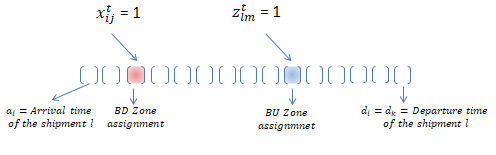
\includegraphics[width=130mm,scale=1.5]{Marco_2.png}
	\caption{Journey of Shipment - 2}
	\label{fig:Journey of Shipment - 2}
\end{figure}

The end time of ULD i in Break down process and the summation of transportation time needed to reach Warehouse shall be less that the time at which the shipment l is assigned to a workstation 'm' in Build up zone of flight k.
\begin{align}
 \sum_{j \in J}\sum_{t=a_{l}}^{d_{i}}{\color{black}{(t + h_{j} + T_{j})}} . x_{ij}^t  \le \sum_{m \in M_{k}}\sum_{t=a_{l}}^{d_{l}}z_{lm_{k}}^t . t \qquad \forall i \in I , \forall l \in L_{i}
\end{align}

For Multiple DZ ULDs we have to consider only NRML BD zone assignments for writing precedence constraint : 

\begin{align}
 \sum_{j \in J_{NRML}}\sum_{t=a_{l}}^{d_{i}}{\color{black}{(t + h_{j} + T_{j})}} . x_{ij}^t  \le \sum_{m \in M_{k}}\sum_{t=a_{l}}^{d_{l}}z_{lm_{k}}^t . t \qquad \forall i \in I , \forall l \in L_{i}
\end{align}

Slack for each shipment is given by difference in departure time and the time at which shipments are built up into ULDs. Let this slack time for each shipment be greater than ${s_{min}}$

\begin{align}
 ( d_{l} + p_{k}) - (z_{lm_{k}}^t .(t + b_{k}) )  \ge s_{min} \qquad \forall i \in I, \forall l \in L_{i}, \forall k \in K, \forall t \in T
\end{align}
\begin{align}
s_{min} \ge 0
\end{align}

\subsection{Objective Function}
\label{sec:objBUZone}

By maximizing the minimum slack of all shipments, we ensure that each shipment is ready well before its departure time.

\begin{equation*}
\max s_{min}
\end{equation*}


\section{Solving The Problem and The Model Output}
\label{sec:modeloutput}

We implemented all presented models in Jupyter Notebook using Gurobi for Python. It takes three hours to build the entire model. In the solution, we see that all shipments catch their flights on time as our goal in this project. 

$\newline$
To choose a planning time horizon that fits our needs, we evaluated different planning time horizons with repect to the solution quality and the runtime. For the BD zones, first we determined the planning horizon as one minute but it took a lot of time for the solution. Then we decided to discretize the time in handling time intervals for each BD zone. For the BU zones, time is discretized in one minute intervals.

$\newline$
When we analyze the result for the BD zones, we can see in both Figure 5 and Figure ... that most of the shipments are assigned to BD zone called BD NRML-4. Because transportation time and the handling time for this particular BD zone are less than the others. Hence, our model picked the best BD zone. 


\begin{figure}[hbt!]
	\centering
	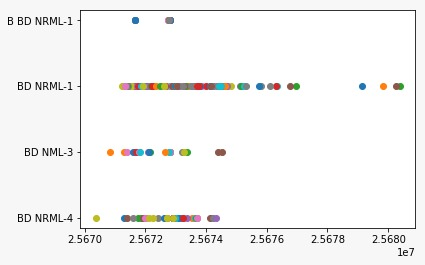
\includegraphics[width=150mm,scale=1.0]{ShipmentArrivalTimeAndBDZones.jpeg}
	\caption{Shipment Arrival Times (X-axis) and BD Zones (Y-axis)}
	\label{fig:Shipment Arrival Times (X-axis) and BD Zones (Y-axis)}
\end{figure}

\begin{figure}[hbt!]
	\centering
	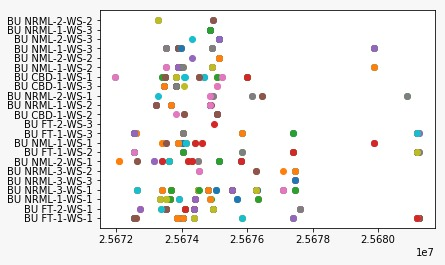
\includegraphics[width=150mm,scale=1.0]{FlightDepTimesAndBUZones.jpeg}
	\caption{Flight Departure Times (X-axis) and BU Zones (Y-axis)}
	\label{fig:Flight Departure Times (X-axis) and BU Zones (Y-axis)}
\end{figure}

%\subsection{Overall Model}
%\label{sec:overallModel}

%------------------------------------------------------------------------

%\begin{table}[h!]
%	\begin{center}
%		\caption{Drop Zone}
%		\label{tab:table1}
%		\begin{tabular}{l|c|c} % <-- Alignments: 1st column left, 2nd middle and 3rd right, with vertical lines in between
%			\textbf{Name} & \textbf{Workstations} & \textbf{Sequence}\\
%			\hline
%			& & \\
%			DZ NRML-1 & 6 & 1\\
%			DZ NRML-2 & 4 & 2\\
%			DZ NML-1 & 3 & 3\\
%			DZ CLD-1 & 5 & 4\\
%		\end{tabular}
%	\end{center}
%\end{table}

%\begin{table}[h!]
%	\begin{center}
%		\caption{Break Down Zone}
%		\label{tab:table1}
%		\begin{tabular}{l|c|c|c|c} % <-- Alignments: 1st column left, 2nd middle and 3rd right, with vertical lines in between
%			\textbf{Name} & \textbf{Workstations} & \textbf{Sequence} & \textbf{ToWH} & \textbf{HandTimePerULD}\\
%			\hline
%			& & & & \\
%			B BD NRML-1 & 33 & 1 & 0:30 & 0:24\\
%			B BD NRML-2 & 10 & 2 &  0:25 & 0:24\\
%			BD NML-1 & 4 & 3 &  0:40 & 0:13\\
%			BD CLD-1 & 8 & 4  &  0:30 & 0:17\\
%			BD NRML-1 & 5 & 5  &  0:30 & 0:20\\
%			BD NML-2 & 3 & 6  & 0:25 & 0:13\\
%			BD NRML-2 & 6 & 7  & 0:40 & 0:20\\
%			BD NRML-3 & 3 & 8  & 0:40 & 0:20\\
%			BD CLD-2 & 5 & 9  & 0:30 & 0:17\\
%			BD NML-3 & 5 & 10  & 0:25 & 0:20\\
%			BD NRML-4 & 3 & 11  & 0:30 & 0:13\\
%			BD CLD-4 & 1 & 12  & 0:40 & 0:15\\
%		\end{tabular}
%	\end{center}
%\end{table}

\end{document}